\documentclass[a4paper, 12pt]{article}
\usepackage{temp}
\usepackage{epsfig,graphicx,subfigure,amsthm,amsmath, float, xcolor, changepage, mathtools, textcomp, hyperref, bm, amssymb, tcolorbox, tikz, setspace}
\usepackage{array}
\usepackage[shortlabels]{enumitem}
\usepackage[bottom]{footmisc}
\usepackage{xepersian}
\settextfont[Scale=1]{XBZar}
%\setdigitfont{XBZar}
\setlatintextfont[Scale=0.9]{Times New Roman}
\hypersetup{
	colorlinks=true,
	urlcolor=blue!70!black
}

\newcolumntype{?}{!{\vrule width 1pt}}

\doublespacing
\begin{document}
\handout
{هوش مصنوعی}
{نیم‌سال اول
۱۴۰۱\lr{-}۱۴۰۰}
{دکتر محمدحسین رهبان}
{دانشکده مهندسی کامپیوتر}
{مینی‌پروژه سوم - تئوری}
{محمدجواد هزاره}
{98101074}
\noindent
\\[-6em]
\section*{سوال ۱}
\begin{enumerate}[A)]
	\item
	در هر دو مورد حرکت مجازی باقی‌مانده است که با یال رنگ شده در تصاویر زیر نشان داده شده است:
	\begin{center}
		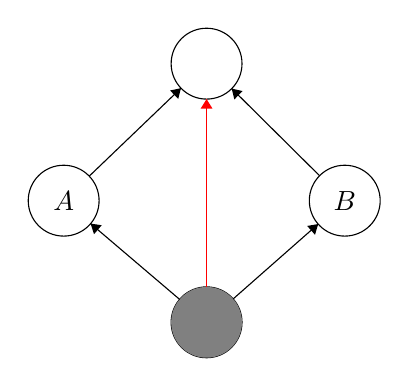
\begin{tikzpicture}[scale=0.15]
			\tikzstyle{every node}+=[inner sep=0pt]
			\draw [black] (38.9,-17.6) circle (3);
			\draw [black] (38.9,-39.5) circle (3);
			\fill [gray] (38.9,-39.5) circle (3);
			\draw [black] (50.6,-29.2) circle (3);
			\draw (50.6,-29.2) node {$B$};
			\draw [black] (26.8,-29.2) circle (3);
			\draw (26.8,-29.2) node {$A$};
			\draw [black] (41.15,-37.52) -- (48.35,-31.18);
			\fill [black] (48.35,-31.18) -- (47.42,-31.34) -- (48.08,-32.09);
			\draw [black] (36.62,-37.56) -- (29.08,-31.14);
			\fill [black] (29.08,-31.14) -- (29.37,-32.04) -- (30.02,-31.28);
			\draw [black] (28.97,-27.12) -- (36.73,-19.68);
			\fill [black] (36.73,-19.68) -- (35.81,-19.87) -- (36.5,-20.59);
			\draw [black] (48.47,-27.09) -- (41.03,-19.71);
			\fill [black] (41.03,-19.71) -- (41.25,-20.63) -- (41.95,-19.92);
			\draw [red] (38.9,-36.5) -- (38.9,-20.6);
			\fill [red] (38.9,-20.6) -- (38.4,-21.4) -- (39.4,-21.4);
		\end{tikzpicture}
		\hspace*{3em}
		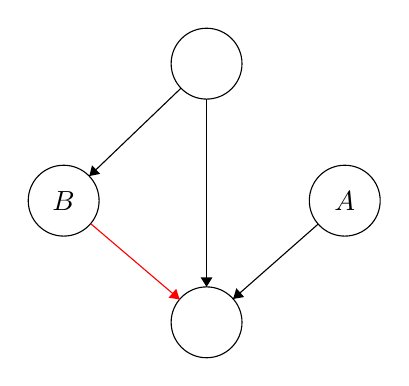
\begin{tikzpicture}[scale=0.15]
			\tikzstyle{every node}+=[inner sep=0pt]
			\draw [black] (38.9,-17.6) circle (3);
			\draw [black] (38.9,-39.5) circle (3);
			\draw [black] (50.6,-29.2) circle (3);
			\draw (50.6,-29.2) node {$A$};
			\draw [black] (26.8,-29.2) circle (3);
			\draw (26.8,-29.2) node {$B$};
			\draw [black] (48.35,-31.18) -- (41.15,-37.52);
			\fill [black] (41.15,-37.52) -- (42.08,-37.36) -- (41.42,-36.61);
			\draw [red] (29.08,-31.14) -- (36.62,-37.56);
			\fill [red] (36.62,-37.56) -- (36.33,-36.66) -- (35.68,-37.42);
			\draw [black] (38.9,-20.6) -- (38.9,-36.5);
			\fill [black] (38.9,-36.5) -- (39.4,-35.7) -- (38.4,-35.7);
			\draw [black] (36.73,-19.68) -- (28.97,-27.12);
			\fill [black] (28.97,-27.12) -- (29.89,-26.93) -- (29.2,-26.21);
		\end{tikzpicture}
	\end{center}
	\item
\end{enumerate}
\section*{سوال ۲}
\begin{itemize}
	\item
	تبدیل فاکتورها به صورت زیر خواهد بود:
	\[
	\begin{aligned}
		B:\quad&\prob(B|G),\quad \prob(B|D),\quad \prob(B|E) && \longrightarrow  f_1(D,G,E) \\
		E:\quad&\prob(E), \quad f_1(D,G,E) && \longrightarrow f_2(D,G) \\
		D:\quad&\prob(D|G), \quad \prob(D|H), \quad \prob(A|D), \quad f_2(D,G) && \longrightarrow f_3(A,H,G) \\
		C:\quad&\prob(C|F), \quad \prob(C|I), \quad \prob(A|C) && \longrightarrow f_4(A,F,I) \\
		H:\quad&\prob(H|I), \quad \prob(F|H), \quad \prob(G|H), \quad f_3(A,H,G) && \longrightarrow f_5(A,F,G,I) \\
		I:\quad&\prob(I), \quad f_4(A,F,I), \quad f_5(A,F,G,I) && \longrightarrow f_6(A,F,G)		
	\end{aligned}
	\]
	\item
	تبدیل فاکتورها به صورت زیر است:
	\[
	\begin{aligned}
		I:\quad&\prob(I),\quad\prob(H|I),\quad\prob(C|I) &&\longrightarrow f_1(H,C) \\
		H:\quad&\prob(F|H),\quad\prob(D|H),\quad\prob(G|H),\quad f_1(H,C) &&\longrightarrow f_2(F,D,G,C) \\
		C:\quad&\prob(C|F),\quad\prob(A|C),\quad f_2(F,D,G,C) &&\longrightarrow f_3(A,F,D,G) \\
		D:\quad&\prob(D|G),\quad\prob(A|D),\quad f_3(A,F,D,G) &&\longrightarrow f_4(A,F,G) \\
		E:\quad&\prob(E),\quad\prob(B|E) &&\longrightarrow f_5(B) \\
		B:\quad&\prob(B|G),\quad f_5(B) &&\longrightarrow f_6(G)
	\end{aligned}
	\]
\end{itemize}
ترتیب دوم برای پاسخ به پرسمان داده شده مناسب‌تر است چرا که زودتر به فاکتور موردنظر رسیده‌ایم (در مرحله‌ی حذف $D$ به این فاکتور رسیده‌ایم.)
\section*{سوال ۳}
\begin{enumerate}[A)]
	\item
	اگر احتمال سرگیجه داشتن را با $p$ نشان دهیم، آن‌گاه احتمال نرمال بودن برابر $1-p$ خواهد بود و داریم:
	\[
	p = p\times 0.3 + (1-p)\times 0.1
	\]
	که با حل معادله‌ی بالا برای $p$ خواهیم داشت:
	\[
	p = \frac{1}{8}
	\]
	\item
	هدف پیدا کردن احتمال هر یک از بیماری‌های مذکور به شرط آن است که بدانیم بیمار دچار سرگیجه‌ی مزمن و تنگی نفس هست. برای احتمال ضعف عظلات قلب داریم:
	\[
	\prob(X=H|S=1, D=1) = \frac{1}{Z} \,\prob(X=H, S=1, D=1)
	\]
	که $Z$ فاکتور نرمال‌کننده‌ی احتمال است. برای احتمال مشترک نیز داریم:
	\[
	\begin{aligned}
		\prob(X=H, S=1, D=1) &= \sum_{y}\prob(X=H, y, S=1, D=1) \\
		&= \sum_{y} \prob(X=H)\prob(S=1|X=H)\prob(y|X=H)\prob(D=1|y) \\
		&= \prob(X=H)\prob(S=1|X=H)\prob(Y=bd|X=H)\prob(D=1|Y=bd) \\
		&\quad\qquad + \prob(X=H)\prob(S=1|X=H)\prob(Y=bc|X=H)\prob(D=1|Y=bc) \\
%		&\quad\qquad + \prob(X=H)\prob(S=0|X=H)\prob(Y=bc|X=H)\prob(D=1|Y=bc) \\
%		&\quad\qquad + \prob(X=H)\prob(S=1|X=H)\prob(Y=bc|X=H)\prob(D=1|Y=bc) \\
		&= (0.02 \times 0.5 \times 0.7 \times 0.8) + (0.02 \times 0.5 \times 0.1 \times 0.7) \\
%		&\quad\qquad + (0.02 \times 0.5 \times 0.1 \times 0.7) + (0.02 \times 0.5 \times 0.1 \times 0.7)\\
		&= 6.3 \times 10^{-3}
	\end{aligned}
	\]
	احتمال بیماری \lr{sepsis} نیز به طور مشابه برابر با
	\[
	\prob(X=S|S=1, D=1) = \frac{1}{Z} \,\prob(X=S, S=1, D=1)
	\]
	که $Z$ همان فاکتور نرمال‌کننده‌ی حالت قبل است. برای احتمال مشترک به طور مشابه داریم:
	\[
	\begin{aligned}
		\prob(X=S, S=1, D=1) &= \sum_{y}\prob(X=S, y, S=1, D=1) \\
		&= \sum_{y} \prob(X=S)\prob(S=1|X=S)\prob(y|X=S)\prob(D=1|y) \\
		&= \prob(X=S)\prob(S=1|X=S)\prob(Y=bd|X=S)\prob(D=1|Y=bd) \\
		&\quad\qquad + \prob(X=S)\prob(S=1|X=S)\prob(Y=bc|X=S)\prob(D=1|Y=bc) \\
%		&\quad\qquad + \prob(X=S)\prob(S=0|X=S)\prob(Y=bc|X=S)\prob(D=1|Y=bc) \\
%		&\quad\qquad + \prob(X=S)\prob(S=1|X=S)\prob(Y=bc|X=S)\prob(D=1|Y=bc) \\
		&= (0.003 \times 0.85 \times 0.7 \times 0.8) + (0.003 \times 0.85 \times 0.5 \times 0.7) \\
%		&\quad\qquad + (0.003 \times 0.15 \times 0.5 \times 0.7) + (0.003 \times 0.85 \times 0.5 \times 0.7)\\
		&= 2.3 \times 10^{-3}
	\end{aligned}
	\]
	بنابراین احتمال این‌که بیماری موردنظر ضعف عظلات قلب باشد بیش‌تر است.
\end{enumerate}
\end{document}



